% https://github.com/dreading/tex-neural-network
% https://medium.com/momenton/typesetting-neural-network-diagrams-with-tex-4920b6b9fc19

\documentclass{article}

% Preamble
\usepackage{tikz}
\usetikzlibrary{matrix,chains,positioning,decorations.pathreplacing,arrows}

\begin{document}

 % Listing 1: Tex for neural network layers
\begin{figure}

    \centering
    
    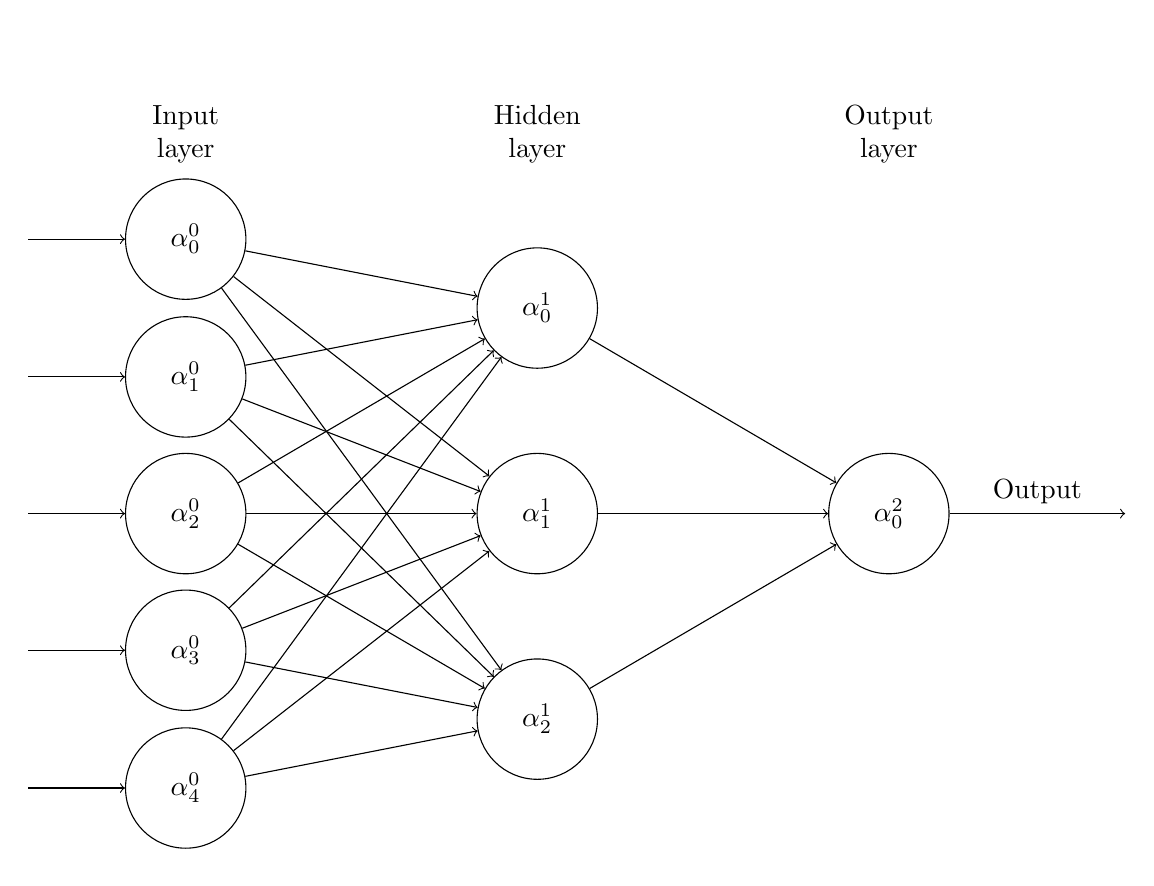
\begin{tikzpicture}[
         % define styles 
          clear/.style={
          draw=none,
          fill=none,
          },
        net/.style={
          matrix of nodes,
          nodes={
               draw,
               circle,
               inner sep=10pt
          },
          nodes in empty cells,
          column sep=2cm,
          row sep=-19pt
          } 
    ]
        % define matrix mat to hold nodes
        % using net as default style for cells
        \matrix[net] (mat)
        {
            % Define layer headings
            |[clear]| \parbox{1.3cm}{\centering Input\\layer} 
              & |[clear]| \parbox{1.3cm}{\centering Hidden\\layer} 
              & |[clear]| \parbox{1.3cm}{\centering Output\\layer} \\
         
            $\alpha_{0}^{0}$  & |[clear]|        & |[clear]| \\
            |[clear]|         & $\alpha_{0}^{1}$ & |[clear]| \\
            $\alpha_{1}^{0}$  & |[clear]|        & |[clear]| \\
            |[clear]|         & |[clear]|        & |[clear]| \phantom{$\alpha_{0}^{0}$} \\
            $\alpha_{2}^{0}$  & $\alpha_{1}^{1}$ & $\alpha_{0}^{2}$ \\
            |[clear]|         & |[clear]|        & |[clear]|  \phantom{$\alpha_{0}^{0}$} \\
            $\alpha_{3}^{0}$  & |[clear]|        & |[clear]| \\
            |[clear]|         & $\alpha_{2}^{1}$ & |[clear]| \\
            $\alpha_{4}^{0}$  & |[clear]|        & |[clear]| \\ 
        };
        
        
        % left most lines into input layers
        \foreach \ai in {2,4,...,10}
            \draw[<-] (mat-\ai-1) -- +(-2cm,0);
        
        % lines from a_{i}^{0} to each a_{j}^{1}
        \foreach \ai in {2,4,...,10} {
            \foreach \aii in {3,6,9}
                \draw[->] (mat-\ai-1) -- (mat-\aii-2);
                }
        
        % lines from a_{i}^{1} to a_{0}^{2}
        \foreach \ai in {3,6,9}
          \draw[->] (mat-\ai-2) -- (mat-6-3);
            
        % right most line with Output label
        \draw[->] (mat-6-3) -- node[above] {Output} +(3cm,0);
        
    \end{tikzpicture}
    
    \caption{Neural network layers}
    
\end{figure}


% Listing 2: Tex for neural network pipeline
\begin{figure}
    \centering
    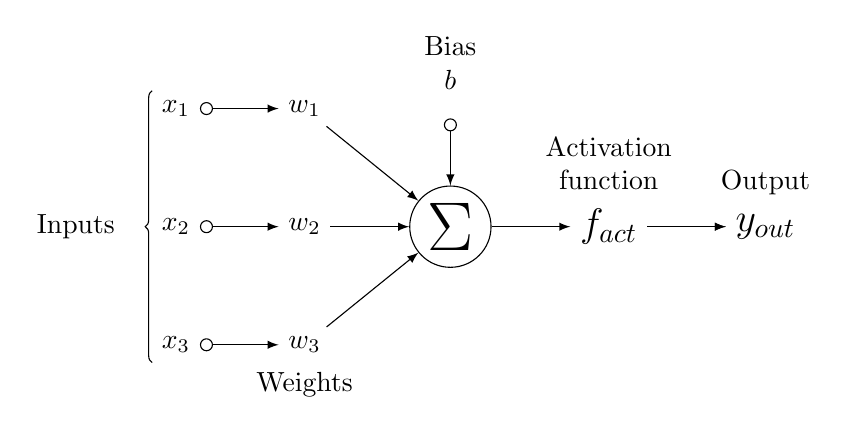
\begin{tikzpicture}[
        % define styles    
        init/.style={ 
             draw, 
             circle, 
             inner sep=2pt,
             font=\Huge,
             join = by -latex
        },
        squa/.style={ 
            font=\Large,
            join = by -latex
        }
    ]
        
        % Top chain x1 to w1
        \begin{scope}[start chain=1]
            \node[on chain=1] at (0,1.5cm)  (x1) {$x_1$};
            \node[on chain=1,join=by o-latex] (w1) {$w_1$};
        \end{scope}
        
        % Middle chain x2 to output
        \begin{scope}[start chain=2]
            \node[on chain=2] (x2) {$x_2$};
            \node[on chain=2,join=by o-latex] {$w_2$};
            \node[on chain=2,init] (sigma) {$\displaystyle\Sigma$};
            \node[on chain=2,squa,label=above:{\parbox{2cm}{\centering Activation\\ function}}]   {$f_{act}$};
            \node[on chain=2,squa,label=above:Output,join=by -latex] {$y_{out}$};
        \end{scope}
        
        % Bottom chain x3 to w3
        \begin{scope}[start chain=3]
            \node[on chain=3] at (0,-1.5cm) 
            (x3) {$x_3$};
            \node[on chain=3,label=below:Weights,join=by o-latex]
            (w3) {$w_3$};
        \end{scope}
        
        % Bias
        \node[label=above:\parbox{2cm}{\centering Bias \\ $b$}] at (sigma|-w1) (b) {};
        
        % Arrows joining w1, w3 and b to sigma
        \draw[-latex] (w1) -- (sigma);
        \draw[-latex] (w3) -- (sigma);
        \draw[o-latex] (b) -- (sigma);
        
        % left hand side brace
        \draw[decorate,decoration={brace,mirror}] (x1.north west) -- node[left=10pt] {Inputs} (x3.south west);
        
    \end{tikzpicture}
    
    \caption{Neural network pipeline}
    
\end{figure}


\end{document}